\section{What the 50 ms reading adds at 100 ms}
\label{sec:coverage}

\subsection{Paired forecasts at a common deadline}
At 100 ms both aerodynamic predictors know the latest ball position. We give one of them the 50 ms reading as well. Both start computing at 100 ms with the same priors, force laws and solver. Each draws 8,192 proposals per force model, propagates up to 512 positive-weight samples per model and reports the centre of the most probable goal cell. A gravity-only control uses both readings, predicts a continuous ballistic crossing and assigns direct entry a probability of zero or one.

We generated 90 calibration kicks and 120 test kicks with fresh random seeds. The reference solver used a 1 ms step and different force laws from the predictor, with balanced blocks of zero-spin, stable-spin and low-spin wake trajectories (Appendix~\ref{app:reference}). We calibrated the regions on 55 direct entries and scored locations on the 71 test entries. All 120 test kicks contributed to the event scores.

We rounded each kick's exact coordinates to the nearest centimetre. For a second set of readings, we first added independent Gaussian errors in each frame (6 mm standard deviation per coordinate) and a Gaussian bias shared by both frames (8 mm standard deviation per coordinate). Release position and frame times were exact in both sets. For noisy readings the predictor used the same error model as the generator. Appendix~\ref{app:event} treats timing errors separately.

We prespecified the three methods, coverage targets from 50 to 100\% (90\% for the main comparison), and subgroups by spin family and distance from the goal edge. Each kick used one inference seed across methods and measurement conditions. The predictor saw only the input positions. We saved and hashed its forecasts before scoring them against the references.

\subsection{Calibrating regions on the goal grid}
For each method and measurement condition, calibration sets a threshold for including cells. In the aerodynamic forecasts, rank the grid cells \(j_1,\ldots,j_J\) by decreasing probability \(H_D(j)\) conditional on direct entry, breaking ties in a fixed order. The score of an occupied cell is the mass of the cells ahead of it,
\begin{equation}
 S_D(j_k)=\sum_{\ell<k}H_D(j_\ell).
 \label{eq:coverage-prefix}
\end{equation}
An empty cell scores one. For gravity, a cell whose centre lies distance \(d_j\) from the ballistic crossing scores \(d_j/(L+d_j)\), where \(L\) is the goal diagonal. Thresholding this score amounts to choosing a radius about the crossing. If the map or ballistic crossing is unavailable, every cell receives a score of one.

For a target coverage \(c\), sort the scores of the 55 true calibration cells and take the \(\lceil(55+1)c\rceil\)-th smallest as \(q_c\). Include all cells with \(S_D(j)\le q_c\). If the rank exceeds 55, set \(q_c=1\). Whenever \(q_c=1\), the region covers the whole goal. This split-calibration rule gives marginal coverage under exchangeability~\cite{lei}. Our test measures the hit rate on the specified, block-balanced synthetic population. Coverage on real kicks requires independent field data.

\begin{table}[htbp]
\centering\small
\caption{Forecasts at the 90\% calibration target. Hits, mean area and mean point error use the 71 direct entries. The Brier score for direct entry uses all 120 test kicks. The gravity control uses both readings and a calibrated radius.}
\label{tab:z09main}
\begin{tabular}{@{}llrrrr@{}}\toprule
Profile & Forecast & Hits & Area (m\(^2\)) & Mean error (m) & Brier\\\midrule
\csname @@input\endcsname tables/coverage-main.tex
\bottomrule\end{tabular}
\end{table}

\begin{figure}[htbp]\centering
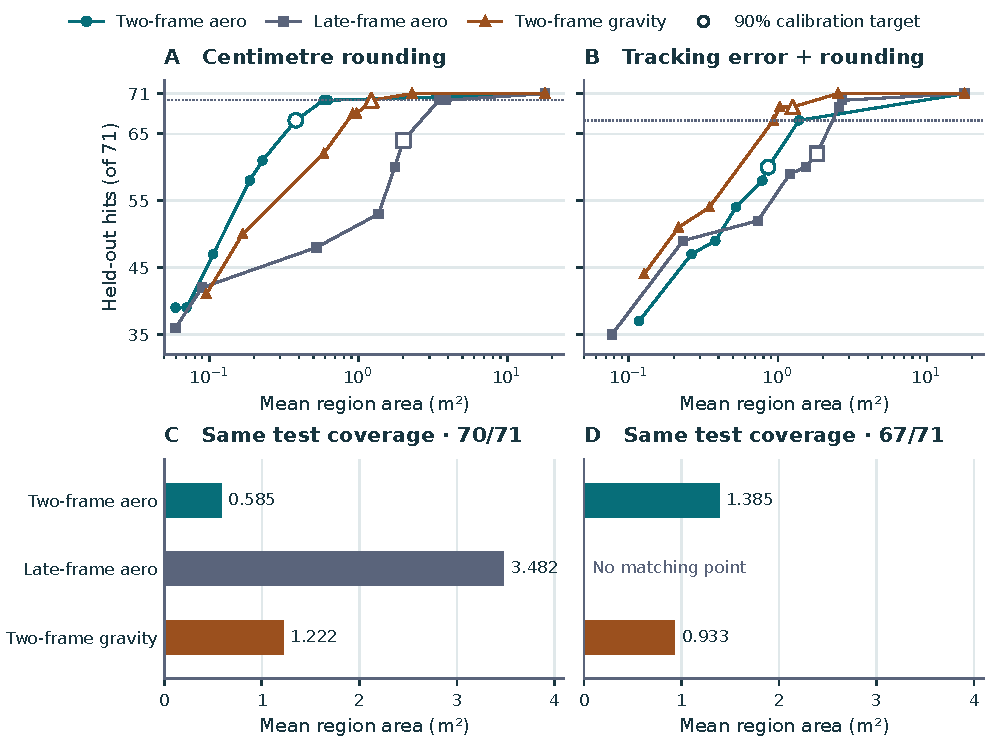
\includegraphics[width=\linewidth]{coverage-frontier.pdf}
\caption{\textbf{Goal area at matched test coverage.} Panels A and B plot hits against mean area on a log scale for the same 71 direct entries. Open markers denote the 90\% calibration target. Panels C and D compare prespecified thresholds that yielded equal hit counts. The late-frame curve has no sampled point at 67/71 hits. The full opening spans \(17.86\ \mathrm{m^2}\).}
\label{fig:frontier}
\end{figure}

\subsection{The early frame narrows the region under centimetre rounding}
At the 90\% target, two frames covered 67/71 entries in \(0.381\ \mathrm{m^2}\) on average, compared with 64/71 in \(2.003\ \mathrm{m^2}\) using the late frame alone (Table~\ref{tab:z09main}). The respective 95\% Wilson intervals for coverage were 86.4--97.8\% and 81.0--95.1\%. At their 95\% targets, both methods covered 70/71 entries. The two-frame region averaged \(0.585\ \mathrm{m^2}\), compared with \(3.482\ \mathrm{m^2}\) for the late frame. Gravity covered 70/71 in \(1.222\ \mathrm{m^2}\) at its 90\% target (Fig.~\ref{fig:frontier}). Equal counts can include different kicks.

Adding the early frame lowered point error on 13 entries, left it unchanged on 54 and raised it on four (Fig.~\ref{fig:paired-error}). The mean reduction was 3.80 cm (95\% interval 0.22--7.62 cm from 4,000 paired resamples of kicks). The mean reduction relative to gravity had a 95\% interval of \(-2.29\) to \(5.85\) cm. The Brier score for direct entry was 0.018 with both frames, 0.070 with the late frame and 0.083 for the binary gravity forecast.

\subsection{Tracking error changes which forecast is more precise}
At the same 90\% target, the two-frame region was the smallest but covered only 60/71 noisy crossings, compared with 62/71 for the late frame and 69/71 for gravity. All eleven misses by the two-frame forecast came from the stable-spin group (12/23 hits). It covered 24/24 in each of the zero-spin and wake groups. Gravity covered 21/23 stable-spin entries (Table~\ref{tab:subgroup}).

At 67/71 observed hits, gravity used \(0.933\ \mathrm{m^2}\) at its 80\% target and two-frame aerodynamics used \(1.385\ \mathrm{m^2}\) at its 95\% target. These two targets yielded equal coverage on this particular test sample. For the 71 direct entries, the aerodynamic grid centre had a mean point error 5.57 cm larger than the continuous gravity forecast (paired 95\% interval 1.17--10.25 cm). The intervals for both the point-error and Brier-score differences between two-frame and late-frame aerodynamics included zero.

Estimating acceleration from the readings divides the second position difference by \(h^2\), with \(h=50\) ms. A bias shared by the two frames survives in that difference when the release position is fixed independently (Eq.~\eqref{eq:noise}). Gravity fixes the acceleration. Its relative precision here is consistent with the difficulty of estimating transverse curvature from noisy readings, even when the noise model is known.

\begin{figure}[htbp]\centering
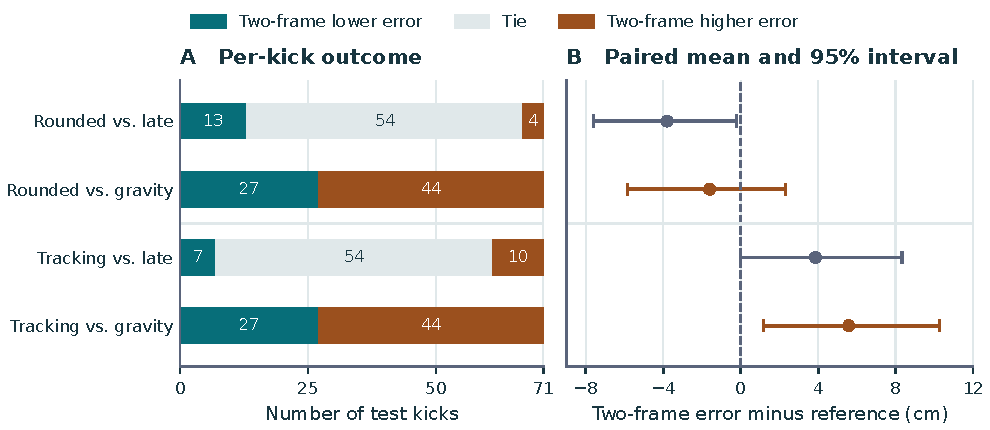
\includegraphics[width=\linewidth]{paired-error.pdf}
\caption{\textbf{Point errors on the same 71 direct-entry kicks.} A counts kicks on which two-frame aerodynamics has a smaller, equal or larger error than each comparison method. B shows the mean paired difference and its 95\% shot-bootstrap interval. Negative values favour two-frame aerodynamics.}
\label{fig:paired-error}
\end{figure}

\subsection{Forecast availability and computation time}
Each method produced a point for all 71 direct entries and an event probability for all 120 kicks under both measurement conditions. Only one run, a noisy late-frame forecast, fell below 25 effective samples. Even with a defined point, the noisy two-frame region filled the entire goal at its 97.5\% target. Appendix~\ref{app:operating} gives the counts near the goal edge.

In the local Python run, two-frame inference and goal-map construction took 84 ms at the median and 94 ms at the 95th percentile with rounding alone. With tracking errors the times were 121 and 131 ms. At the test sampling budget, 131 ms is about 44\% of the nominal 299 ms remaining after the last reading. Capture, reconstruction, transfer and goalkeeper movement require additional time, and the crossing time varies by kick.
